\section{Introduction}

\begin{itemize}
\item Making sense of data-driven claims is hard, even if the evidence base (code/data) is open
\item We see this in peer review, misinformation, retracted papers, …
\end{itemize}

\begin{figure}[h]
   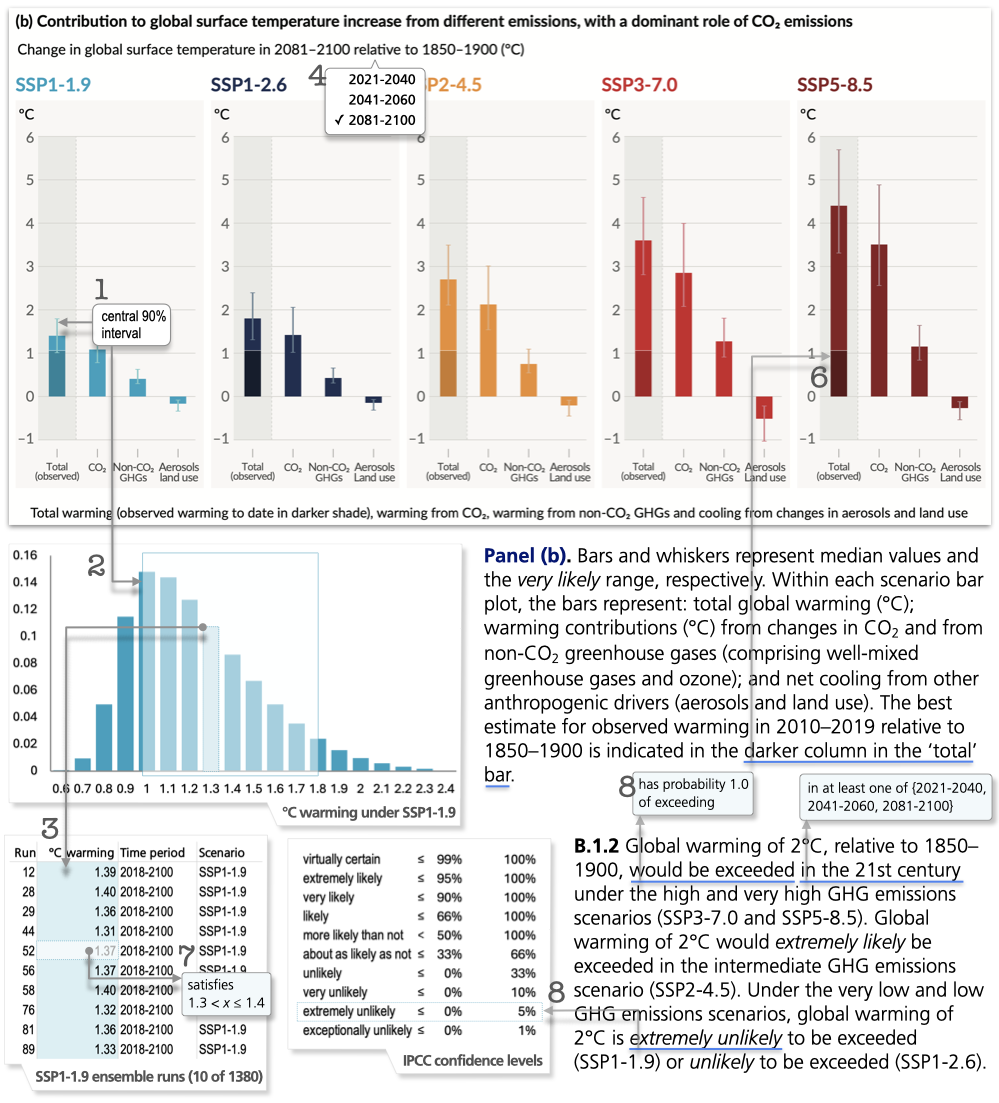
\includegraphics[width=0.9\textwidth]{fig/ipcc-mockup.png}
   \caption{Mockup of end-user transparency features (numbered 1 to 8)}
   \label{fig:ipcc-mockup}
\end{figure}

\subsection{Self-Certifying Text}

\begin{itemize}
\item Introduce basic idea, as complementary to transparent visualisations
\end{itemize}

\subsubsection{Use cases}
Two potential scenarios for this sort of technology:

\paragraph{Authoring transparent text.} Someone authoring content for an online article, wants to create text
linked to raw data (and derivative data such as charts or tabular summaries), so that the evidence base for
the claims made in the text can be explored \emph{in situ}, by interacting with the text.

\paragraph{Interpreting text after the fact.} Someone reading textual claims derived from open data (e.g. a
scientific paper or climate report), wants to retroactively link the text to queries over the available data
and gradually ``rationally reconstruct'' the relationship between the claims in the paper and the evidence
base. Perhaps just to aid their own comprehension, or to provide some kind of justified peer review.

\subsubsection{Idiomatic uses of natural language we might interpret in this way}

Examples of text we might want to link or interpret semi-formally/quantitatively:

\begin{itemize}
\item quantitative expressions
\begin{itemize}
   \item pure numerical values
   \item percentages
   \item rounded or normalised numbers
\end{itemize}
\item graded Adjectives (e.g.~\emph{virtually certain}, \emph{exceptionally unlikely})
\item references to visual elements and their parts (mereology)
\end{itemize}
